\exercisesheader{}

% 1

\eoce{\qt{Migraine and acupuncture,
    Part 1\label{migraine_and_acupuncture_intro}}
A migraine is a particularly painful type of headache,
which patients sometimes wish to treat with acupuncture.
To determine whether acupuncture relieves migraine 
pain, researchers conducted a randomized controlled study
where 89 females diagnosed with migraine headaches were
randomly assigned to one of two groups:
treatment or control.
43 patients in the treatment group received acupuncture 
that is specifically designed to treat migraines.
46 patients in the control group received placebo acupuncture
(needle insertion at non-acupoint locations).
24 hours after patients received acupuncture, they were asked 
if they were pain free.
Results are summarized in the contingency table
below.\footfullcite{Allais:2011}

\noindent\begin{minipage}[l]{0.4\textwidth}
\begin{tabular}{ll  cc c} 
			                         		&           & \multicolumn{2}{c}{\textit{Pain free}} \\
\cline{3-4}
			                        	 	&			& Yes 	& No 	                  & Total \\
\cline{2-5}
							& Treatment 	& 10	 	& 33		                  & 43 \\
\raisebox{1.5ex}[0pt]{\emph{Group}} & Control	 	& 2	 	& 44 	 	                  & 46 \\
\cline{2-5}
							& Total		& 12		& 77		                  & 89
\end{tabular}
\end{minipage}
\begin{minipage}[c]{0.05\textwidth}
\end{minipage}
\begin{minipage}[c]{0.27\textwidth}
\begin{center}
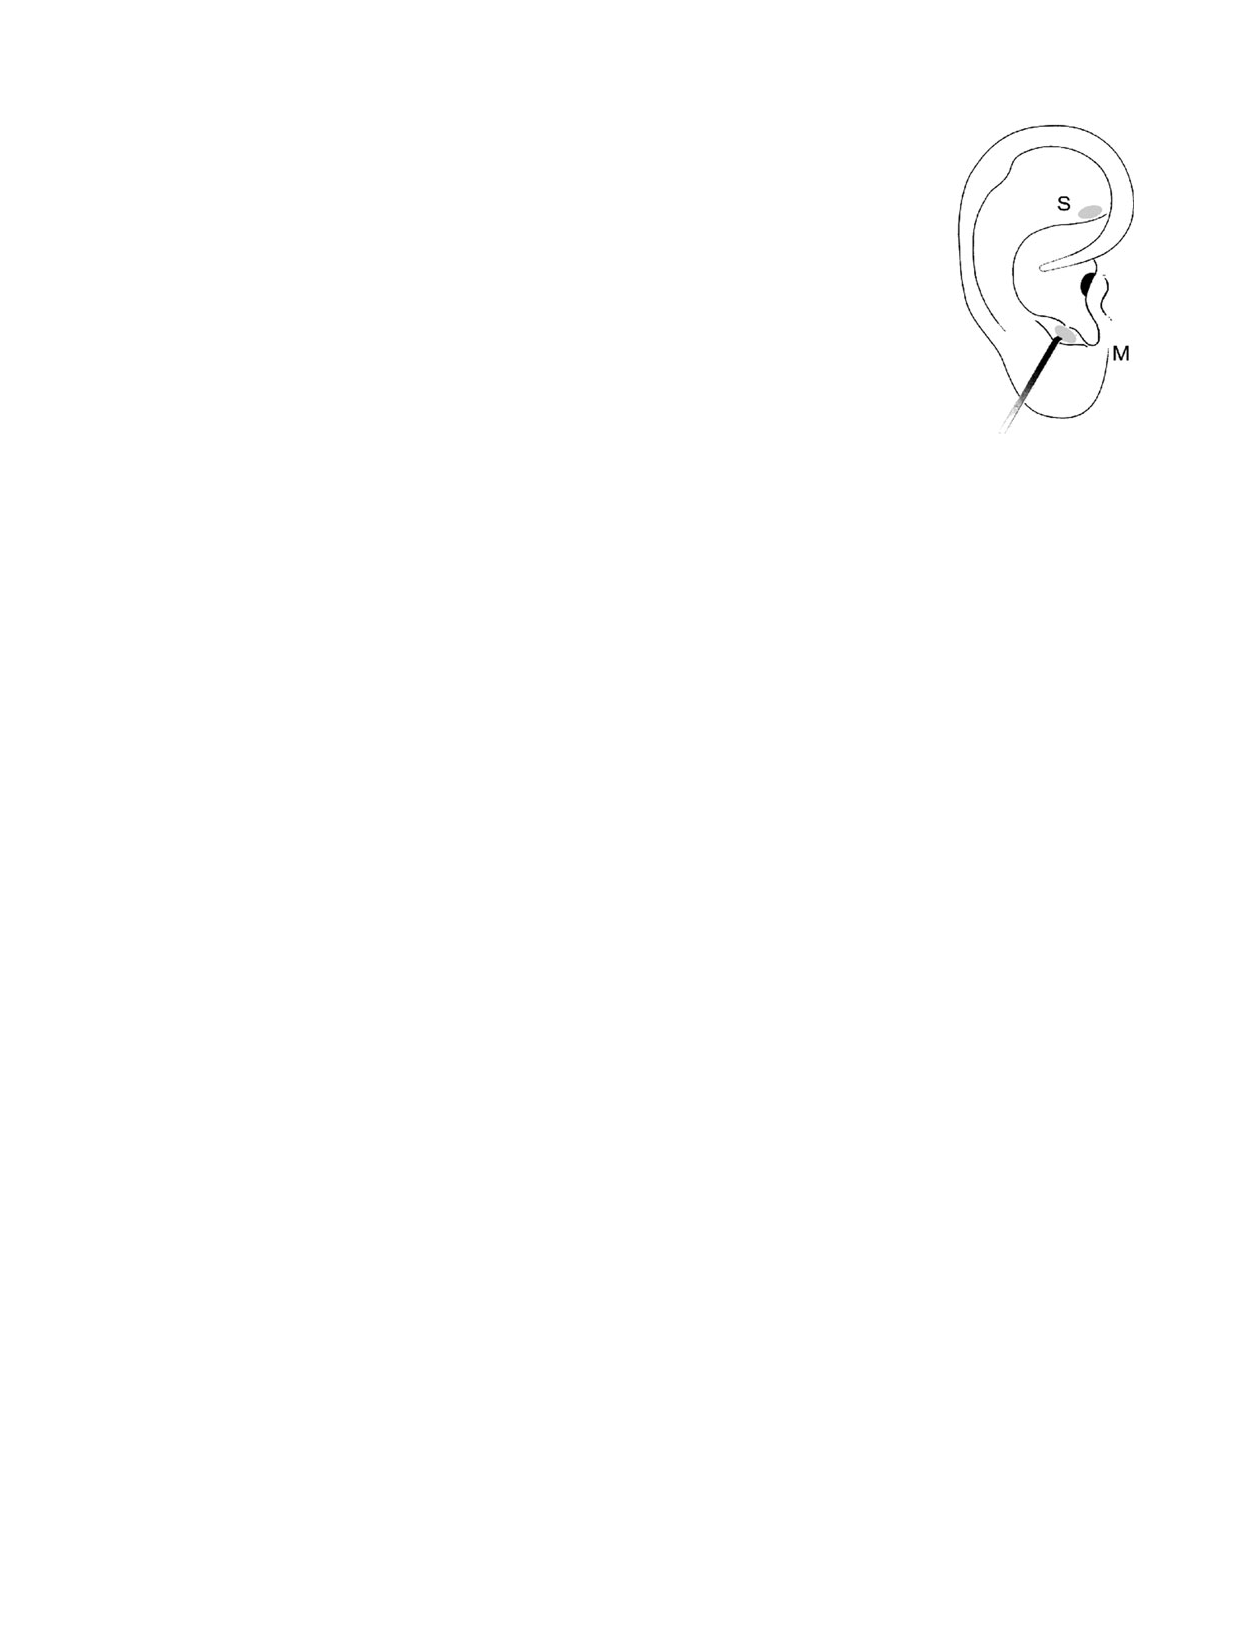
\includegraphics[width = 0.75\textwidth]{ch_data_collection/figures/eoce/migraine_and_acupuncture_intro/earacupuncture.pdf}
\end{center}
\end{minipage}
\begin{minipage}[c]{0.25\textwidth}
{\footnotesize Figure from the original paper displaying the appropriate area 
(M) versus the inappropriate area (S) used in the treatment of migraine attacks.}
\end{minipage}
\begin{parts}
\item What percent of patients in the treatment group were pain free 24 hours 
after receiving acupuncture? 
\item What percent were pain free in the control group?
\item In which group did a higher percent of patients become pain free 24 hours 
after receiving acupuncture?
\item Your findings so far might suggest that acupuncture is an effective treatment 
for migraines for all people who suffer from migraines. However this is not the 
only possible conclusion that can be drawn based on your findings so far. What is 
one other possible explanation for the observed difference between the percentages 
of patients that are pain free 24 hours after receiving acupuncture in the two groups?
\end{parts}
}{}

% 2

\eoce{\qt{Sinusitis and antibiotics,
    Part 1\label{sinusitis_and_antibiotics_intro}} 
Researchers studying the effect of antibiotic treatment for acute sinusitis 
compared to symptomatic treatments randomly assigned 166 adults diagnosed 
with acute sinusitis to one of two groups: treatment or control. Study 
participants received either a 10-day course of amoxicillin (an antibiotic) 
or a placebo similar in appearance and taste. The placebo consisted of 
symptomatic treatments such as acetaminophen, nasal decongestants, etc.
At the end of the 10-day period, patients were asked if
they experienced improvement in symptoms.
The distribution of responses is summarized below. 
\footfullcite{Garbutt:2012}
\begin{center}
\begin{tabular}{ll  cc c} 
                                    			&			& \multicolumn{2}{c}{\textit{Self-reported improvement}} \\
                                    			&			& \multicolumn{2}{c}{\textit{in symptoms}} \\
\cline{3-4}
			                        		&			& Yes 	& No 	& Total \\
\cline{2-5}
							& Treatment 	& 66		& 19		& 85 \\
\raisebox{1.5ex}[0pt]{\emph{Group}}	& Control		& 65		& 16 		& 81 \\
\cline{2-5}
							& Total		& 131	& 35		& 166
\end{tabular}
\end{center}
\begin{parts}
\item What percent of patients in the treatment group experienced improvement 
in symptoms? 
\item What percent experienced improvement in symptoms in the 
control group?
\item In which group did a higher percentage of patients experience improvement
in symptoms?
\item
    Your findings so far might suggest a real difference
    in effectiveness of antibiotic and placebo treatments
    for improving symptoms of sinusitis.
    However, this is not the only possible conclusion that
    can be drawn based on your findings so far.
    What is one other possible explanation for the observed
    difference between the percentages of patients in the
    antibiotic and placebo treatment groups that experience
    improvement in symptoms of sinusitis?
\end{parts}
}{}
